\chapter{Lavori correlati}
\label{cap:nomePrimoCapitoloTesi}
\lhead{\textbf{\rightmark}}

\section{Ricerche correlate}
\label{sec:nomePrimaSezioneCapitolo}
\indent{
	I riferimenti e le ricerche precedenti nella diagnosi del melanoma mobile possono essere suddivisi in tre campi:
	\begin{itemize}
		\item Miglioramento delle tecniche di rilevamento e classificazione del melanoma.
		\item Utilizzo dei dispositivi mobili nei sistemi medici e sviluppo della diagnostica assistita da computer
		\item Miglioramento dei metodi di elaborazione delle immagini per estrarre le caratteristiche del melanoma.
	\end{itemize}
	La ricerca nel primo campo determina i migliori sistemi di machine learning e tecniche di data mining, il secondo campo determina i metodi per costruire il sistema di telemedicina e le possibilità di superare la limitazione mobile nell'elaborazione e archiviazione dei dati utilizzando metodi e algoritmi commisurati alle specifiche mobili.
	\newline
	Il terzo campo è il più importante in questa ricerca, mira a trovare le tecniche di elaborazione delle immagini più accurate per catturare l'immagine e trasformarla in un insieme di funzionalità che possono essere utilizzate nella diagnosi del melanoma.
	\newline
	\newline
	Durante una visita può comparire un melanoma all'ispezione di quattro tipi:
	\newline
	\begin{enumerate}
		\item Melanoma piatto non palpabile: rappresenta la forma più frequente (70\%); tende a crescere verso l'esterno piuttosto che verso l'interno;
		\item Melanoma Cupoliforme o Nodulare: è una variante del melanoma a rapida evoluzione e ad alto rischio di progressione che tende a manifestarsi in età avanzata. Rappresenta il 10-15\% di tutti i melanomi.
		\item Lentigo Maligna (melanoma in situ): è un lento
		lesione in evoluzione che si manifesta come una macchia piatta, non palpabile, marrone, molto liscia, con perdita del normale profilo cutaneo. Generalmente ha un tasso di crescita lento (anni) e raramente si diffonde ad altre parti del corpo.
		\item Melanoma lentigginoso acrale: compare invece nelle zone acrale (palmo della mano, pianta del piede) rappresenta il 5\% di tutti i melanomi. 
	\end{enumerate}
	A causa dell'estrema eterogeneità delle lesioni, è molto difficile identificare e diagnosticare precocemente il melanoma e l'importanza di diagnosticare precocemente il melanoma non è da sottovalutare, questo perché la prognosi nel melanoma è direttamente proporzionale alla profondità della neoplasia.\cite{rigel2010evolution}
	\newline
	Nel 1985 Friedman et al. \cite{friedman1985early} proposero le regole ABCD per creare uno strumento di interpretazione diretto e semplice per i medici.
	\newline
	Successivamente, Abbasi et al. \cite{abbasi2004early} nel 2004 hanno aggiunto la lettera E (per evoluzione) come criterio di riconoscimento per il riconoscimento veloce di una lesione in evoluzione che può essere un melanoma.
	\newline
	L'efficacia del sistema ABCDE è stata convalidata in numerosi studi condotti da dermatologi \cite{carli2005diagnostic}.
	\newline
	\newline
	Le Reti Neurali (RN) rappresentano uno strumento informatico di intelligenza artificiale che ben si adatta alle problematiche clinico-diagnostiche.
	Queste sono state definite per la prima volta in ambito medico già negli anni 90.
	Lo studio di Burke et al. \cite{burke1993applicazione} del 1993, teorizza l'utilizzo delle reti neurali per la medicina di laboratorio ed in particolare per l'analisi delle cellule cancerose.
	\newline
	 Altri due principali esempi di applicazione delle reti neurali, che si trovano descritti, sono uno relativo alla diagnostica radiologica \cite{boone1990neural} e l'altro relativo all'interpretazione dei dati di laboratorio nella diagnosi dei tumori maligni del seno \cite{astion1992application}. Per quanto concerne quest'ultimo, la rete neurale era costituita da nove neuroni in ingresso, quindici neuroni intermedi, e due neuroni in uscita.
	 I nove neuroni in ingresso erano utilizzati per introdurre nella rete i valori assunti dalle nove variabili prescelte: eta' del paziente, la concentrazione nel siero del colesterolo totale, del colesterolo HDL, dei trigliceridi dell'apolipoproteina 
	A-I, dell'apolipoproteina B, dell'albumina, dell'antigene tumorale CA15-3, e l'indice di Fossel (misura dell'ampiezza delle righe dei gruppi metilene e metile nello spettro di risonanza magnetica nucleare protonica).
	 I due neuroni in uscita presentavano i valori di probabilita' (compresa tra 0 e 1) per lo stato di malattia (presenza di tumore maligno del seno) e per lo stato di non malattia (assenza di tumore maligno). 
	 La rete neurale era quindi addestrata mediante la presentazione dei dati relativi a 57 pazienti, di cui 23 con tumore maligno al seno e 34 con affezioni benigne.
	\newline
	\newline
	Per quanto concerne l'analisi dei nevi, in letteratura sono stati presentati diversi sistemi di analisi basati su applicazioni mobile.
	\newline
	Abuzaghleh, et al. \cite{abuzaghleh2014skincure}, hanno presentato un sistema basato su smartphone denominato \textit{SKIN} per assistere la diagnosi precoce del melanoma. Hanno proposto un quadro per analizzare e classificare le immagini di nevi in benigni o possibili melanomi e avvisare l'utente in tempo reale di contattare urgentemente il medico.
	\newline
	Il framework proposto ha confrontato le prestazioni di due tecniche di classificazione:
	\begin{itemize}
		\item Classificatore a un livello;
		\item Classificatore a due livelli;
	\end{itemize}
	Lo studio ha concluso che il classificatore a due livelli supera le prestazioni del classificatore a un livello.
	\newline
	Il paper però non considera alcune informazioni sulla definizione e l'estrazione di caratteristiche (Feature Extraction), ad esempio asimmetria e irregolarità dei bordi, per migliorare l'accuratezza della classificazione.
	\newline
	\newline
	Wadhawan, et al, \cite{wadhawan2011skinscan}, hanno introdotto la libreria portatile SkinScan per il rilevamento del melanoma su dispositivi portatili, una libreria implementata con C/C ++. 
	\newline
	Lo studio ha dimostrato che gli algoritmi più dispendiosi in termini di elaborazione e tempo della libreria, ovvero la segmentazione e la classificazione delle immagini, possono raggiungere una precisione e una velocità di esecuzione paragonabili a un computer desktop. Questi risultati dimostrano che è possibile eseguire applicazioni complesse di imaging biomedico su smartphone e altri dispositivi portatili, che hanno il vantaggio della portabilità.
	Ad ogni modo, il sistema richiede diverso tempo per la segmentazione e la classificazione delle immagini.
	\newline
	\newline
	Ramlakhan et al. \cite{ramlakhan2011mobile}, hanno presentato un prototipo di un sistema di riconoscimento automatizzato del melanoma basato su immagini su smartphone Android, il sistema è costituito da tre componenti principali:
	\begin{itemize}
		\item segmentazione dell'immagine
		\item estrazione delle caratteristiche basata sul metodo ABCD
		\item classificazione
	\end{itemize}
	 Il risultato sperimentale ha mostrato che il sistema non era altamente efficiente ed ha raggiunto una precisione media del 66,7\%, con una sensibilità media della classe maligna del 60,7\% e una specificità dell'80,5\%.
	 \newline
	 Il paper ha presentato due sistemi per la rilevazione di casi di melanoma nelle immagini dermoscopiche utilizzando caratteristiche di consistenza e colore.
	 \newline
	 \newline
	 Karargyris et al. \cite{karargyris2012derma}, hanno lavorato a un'applicazione mobile avanzata di elaborazione delle immagini per il monitoraggio del cancro della pelle. Gli autori hanno presentato un'applicazione per la prevenzione del melanoma, utilizzando un apparato economico (microscopio) e uno smartphone (iPhone). Questi due componenti indipendenti sono sufficienti per acquisire immagini altamente dettagliate per l'utilizzo da parte di esperti con background medico. Inoltre, un framework software avanzato per l'elaborazione delle immagini supporta il sistema per analizzare direttamente le immagini in ingresso.
	 \newline
	 L'obiettivo principale della ricerca era dimostrare come gli smartphone potrebbero trasformarsi in macchine potenti e intelligenti e aiutare grandi popolazioni senza esperienza in contesti con poche risorse. Il loro database di immagini era piccolo e consisteva di sole 6 immagini di casi normali e 6 immagini di casi sospetti.
	 \newline
	 \newline
	 Alcón et. al \cite{alcon2009automatic} hanno descritto un sistema automatico per l'ispezione delle lesioni cutanee pigmentate e la diagnosi del melanoma, che supporta le immagini delle lesioni cutanee acquisite utilizzando una fotocamera digitale convenzionale (di livello commerciale non professionale). Ancora più importante, il sistema creato include una componente di supporto decisionale, che combina il risultato della classificazione dell'immagine con la conoscenza del contesto come il tipo di pelle, l'età, il sesso e la parte del corpo interessata. Ciò consente la stima del rischio personale di melanoma, in modo da aggiungere fiducia alla classificazione. È stato verificato questo sistema classifica le immagini con una precisione dell'86\%, con una sensibilità del 94\% e una specificità del 68\%.
	 \newline
	 L'aggiunta della conoscenza del contesto è stata effettivamente in grado di indicare immagini che sono state erroneamente classificate come benigne, anche se non tutte.
	\section{Applicazioni correlate}
	Nella tecnologia e nelle applicazioni correlate, sono disponibili diverse applicazioni che offrono l'autoesame della pelle e che aiutano l'utente a classificare le lesioni cutanee in benigne o melanomi.
	\newline
	Sulla base della revisione precedente di questa applicazione \cite{wolf2013diagnostic}, le prestazioni delle applicazioni per smartphone nella valutazione del rischio di melanoma sono molto variabili e 3 delle 4 applicazioni per smartphone hanno erroneamente classificato il 30\% o più dei melanomi come benigni.
	\newline
	La revisione mostra che queste applicazioni \textbf{non sono soggette ad alcun tipo di convalida o controllo normativo.} Nonostante le dichiarazioni di non responsabilità secondo cui queste applicazioni sono destinate a scopi educativi, possono danneggiare gli utenti che potrebbero credere erroneamente che la valutazione fornita da tale applicazione sostituisce la consulenza medica. Questo rischio è di particolare preoccupazione per i pazienti economicamente svantaggiati e non assicurati (negli stati ove la sanità è privata). Poiché una percentuale sostanziale di melanomi viene rilevata inizialmente dai pazienti, il potenziale effetto di tali applicazioni sui modelli di rilevamento del melanoma è particolarmente rilevante.
	\newline
	Per queste ragioni, Freeman et al. \cite{freeman2020algorithm} nel 2020 hanno valutato la validità e le scoperte degli studi che esaminano l'accuratezza delle applicazioni per smartphone basate su algoritmi per valutare il rischio di cancro della pelle (melanoma) in lesioni cutanee sospette.
	\newline
	Sono stati inclusi nove studi che hanno valutato sei diverse app per smartphone identificabili. Sei risultati verificati utilizzando l'istologia o il follow-up (n = 725 lesioni) e tre risultati verificati utilizzando le raccomandazioni degli esperti (n = 407 lesioni). Gli studi sono risultati piccoli e di scarsa qualità metodologica, con reclutamento selettivo, alti tassi di immagini inestimabili e verifica differenziale.
	\newline
	La selezione delle lesioni e l'acquisizione delle immagini sono state eseguite dai medici piuttosto che dagli utenti di smartphone. Sono disponibili per il download due app con marchio CE (Conformit Europenne). Non è stato trovato nessuno studio peer review pubblicato sulla valutazione dell'app TeleSkin skinScan. SkinVision è stato valutato in tre studi (n = 267, 66 lesioni maligne o premaligne) e ha raggiunto una sensibilità dell'80\% (intervallo di confidenza 95\% dal 63\% al 92\%) e una specificità del 78\% (dal 67\% all'87\%) per l'individuazione di lesioni maligne o premaligne.
	\begin{figure}[h]
		\begin{center}     
			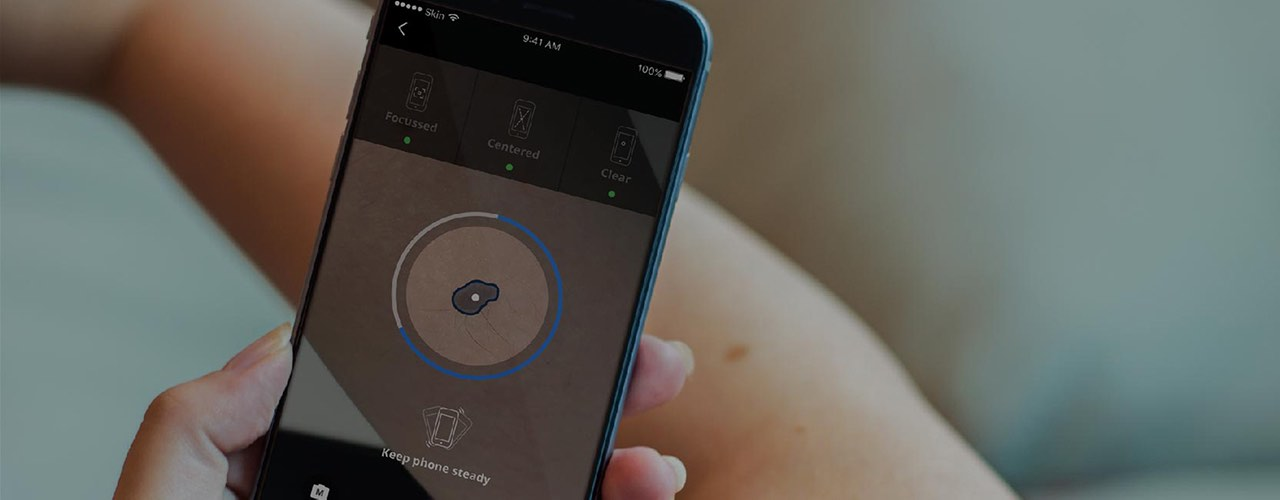
\includegraphics[scale=0.30]{figure/capitolo2/skinvision1.jpg}
		\end{center}
		\caption{Applicazione Skin Vision}	
	\end{figure}
	\newline
	La precisione dell'applicazione SkinVision verificata rispetto alle raccomandazioni degli esperti era scarsa (tre studi).
	\newline
	In conclusione non è possibile fare affidamento sulle attuali applicazioni per smartphone basate su algoritmi (spesso semplificati) per rilevare tutti i casi di melanoma o altri tumori della pelle, perché non applicabili direttamente in un ambito clinico. 
	\newline
	\newline
	Altre applicazioni esistenti sui vari application store, offrono funzionalità simili a quelle presenti in Skin Vision, tra queste è possibile annoverare:
	\newline
\textbf{Medgic} \footnote{Medgic - https://play.google.com/store/apps/details?id=co.medgic.medgic\&gl=IT}, che effettua un analisi e una valutazione ad una foto data input della cute.
	\newline
\textbf{eDerma} \footnote{eDerma - https://play.google.com/store/apps/details?id=com.thenetfirm.android.ederma\&gl=IT}, un' applicazione per il monitoraggio di lesioni cutanee che aiuta a raccogliere informazioni utili per il medico e analizzarne e comprendere l'evoluzione.
Inoltre permette al paziente di poter tenere traccia delle lesioni attraverso un sistema di fotografie passate.
	\begin{figure}[h]
	\begin{center}     
		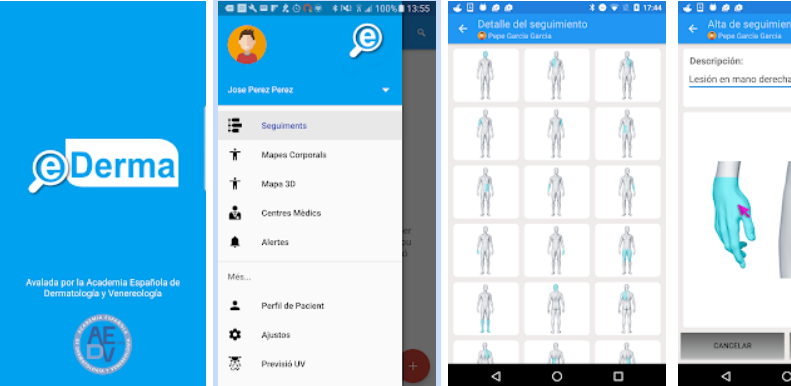
\includegraphics[scale=0.60]{figure/capitolo2/ederma.png}
	\end{center}
	\caption{Applicazione eDerma}	
\end{figure}
\newline
\textbf{Miiskin Skin Tracker} \footnote{Miiskin Skin Traker - https://apps.apple.com/us/app/miiskin-skin-tracker-ehealth/id1214795331} effettua l'imaging automatico della pelle ed utilizza algoritmi di visione artificiale coadivuati con la tecnologia di realtà aumentata per fare il confronto col tempo dei nevi analizzati in passato; questa applicazione però non effettua alcun tipo di diagnosi.
\newline
	Possiamo concludere che le applicazioni di rilevamento del melanoma esistenti presentano diverse carenze sia nell'accuratezza dei risultati sia sull'affidabilità nella diagnosi.
	\newline
	Alcune delle soluzioni proposte costituiscono un pericolo per pazienti, e anche per i dermatologi stessi, che potrebbero essere tratti in inganno dai risultati, quindi abbiamo bisogno di ulteriori ricerche per migliorare l'accuratezza.
	\newline
	Altri sistemi e soluzioni hanno dato buoni risultati in determinati dataset e contesti, ma quando si utilizzano risultati di una camera mobile abbiamo una classificazione imprecisa.
	\newline
	Questi sistemi basati su immagini ad alta risoluzione non sono sempre disponibili. 
	Altri sistemi erano corretti nella diagnosi di alcune delle caratteristiche del melanoma, ma fallivano in altro: ad esempio i risultati erano buoni nel determinare il colore della lesione, ma non riuscivano completamente a identificare proprietà come simmetria e irregolarità.
	\newline
	Attraverso una revisione dei risultati precedenti e dopo aver discusso diversi sistemi, scopriamo che 
	è necessario un lavoro di perfezionamento al fine di perfezionare l'accuratezza dei sistemi, attraverso ulteriori ricerche.
	Allo stesso tempo si può notare come la priorità sembra essere quella di rendere gli algoritmi funzionanti su dispositivi mobili invece di migliorare la precisione degli algoritmi attuali che spesso si basano su immagini raccolte con dermatoscopi professionali, e non tengono conto dell'utilizzo di altri strumenti per la cattura delle immagini di nevi.
	\newline
	\newline
	L'aspetto inerente l'utilizzo della realtà aumentata per l'analisi dei melanomi, in letteratura, ha pochi studi e ricerche, uno studio in particolare di Francese et al.  \cite{francese2020} descrive la possibilità di una applicazione in realtà aumentata che abbia lo scopo di supportare il medico nell'analisi delle lesioni del melanoma visualizzando in realtà aumentata le informazioni fornite.
	In particolare questo modello visibile in Figura prevede:
	\begin{itemize}
		\item Rilevamento della distanza.
		\item Centratura e selezione delle lesioni cutanee. 
		\item Rilevamento ottimale della luce.
		\item Classificatore CNN e parametri di funzionalità.
		\item Creazione della visualizzazione AR.
	\end{itemize}
\begin{figure}[h]
	\begin{center}
		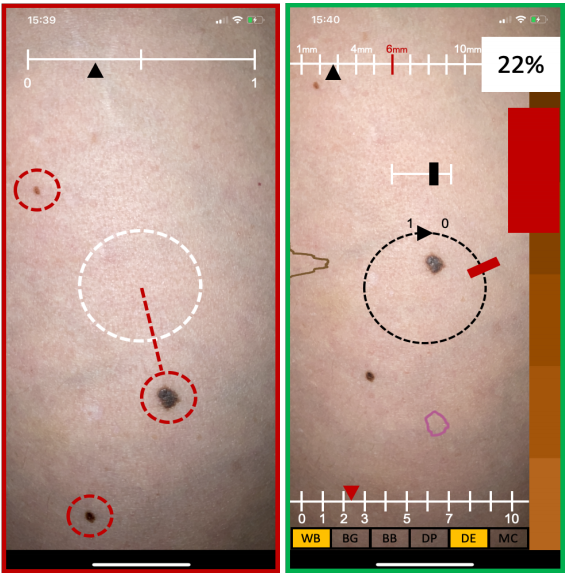
\includegraphics[scale=0.6]{figure/capitolo2/app.png}
	\end{center}
		\caption{Interfaccia proposta dallo studio di Francese et al.}	
\end{figure}
}
